\documentclass[10pt]{article}
% Compile with pdflatex (e.g. on Overleaf). Draft generated from Reading Material/20_Paper_Draft.md;
% every number is traceable to a file in benchmarks/results/ and a command in Reading Material/17.
\usepackage[margin=1in]{geometry}
\usepackage[T1]{fontenc}
\usepackage{lmodern}
\usepackage{booktabs}
\usepackage{graphicx}
\usepackage{amsmath,amssymb}
\usepackage{xcolor}
\usepackage{hyperref}
\usepackage{enumitem}
\setlist{nosep}
\newcommand{\pending}[1]{\textcolor{red}{[pending: #1]}}
\newcommand{\code}[1]{\texttt{#1}}

\title{Making LLM-Guided Program Refinement Reliable:\\
Engine-Side Feedback, Faithful Presentation, and Cross-Prover Certification\\
\large A reproduction study of Refine4LLM with an open model}
\author{Draft --- \textit{authors to be decided}}
\date{October 2026}

\begin{document}
\maketitle

\begin{abstract}
Refine4LLM derives programs from formal specifications by letting a large language model (LLM) choose refinement-calculus laws and their parameters while a prover checks every step, and reports 150/164 verified HumanEval programs passing both the original and the EvalPlus tests. We reimplement the approach with an open-weight model (\code{gpt-oss:120b}, low reasoning effort), Z3 for the search, and Coq and Lean~4 as independent certifiers, and ask how \emph{reliably} such a system succeeds when a run is repeated. On the paper's running example (a square root within an error bound) our first general implementation succeeded in 7 of 10 runs. Every failure we read was caused by what the engine told the model after a failed step---not by the prompt's instructions. Fixing these in the engine with general rules raised the success rate to 99/99 (95\% CI 96--100\%), and the final code to 100/100, with a median of two model calls; the final code solves all 11 further benchmark problems in 20 of 20 runs each (220/220) while never ``proving'' an impossible specification. We further found that the text shown to the model could mean something different from the formula the prover checked, and that the search prover, the certifiers and the executed program disagreed on integer division, float arrays and Booleans; we close each gap and guard it with property tests. Finally we build 20 HumanEval specifications that are checked against the reference solution on every HumanEval and EvalPlus input and mutation-tested, and observe that two 2025 open models \emph{alone} already pass 156/164 and 154/164 (HumanEval) and 147/164 (EvalPlus)---above the paper's GPT-4 baseline---so the contribution of refinement today is the guarantee rather than the pass rate. On those 20 problems the untuned open model derives verified programs reliably only for the simple ones (41 of 121 runs yield a verified, Coq-certified program that passes every test; 7 of 20 problems). Executing the derived programs exposed further gaps between proof and execution, one step that the search prover accepted although it is false---which Coq refused to certify and the tests caught---and a gap in the relaxed termination rule, which admitted a never-ending loop because an integer measure that only has to decrease can decrease for ever; adding the obligation $I\wedge G\Rightarrow 0\le V$ repairs it and keeps the paper's measure admissible.
\end{abstract}

\section{Introduction}
LLMs write plausible code that is sometimes wrong, and tests can show the presence of bugs but not their absence. Refine4LLM~\cite{refine4llm} starts from a specification $x:[P,Q]$, lets the LLM pick a law of Morgan's refinement calculus~\cite{morgan} and its parameters (an intermediate assertion, a guard, a loop invariant and variant), and discharges the law's side condition with a prover. A rejected step returns a counterexample; when every leaf is a primitive statement, the leaves compose into a program that is correct by construction.

The original evaluation reports one run per problem with a fine-tuned GPT-4, a learned law library and Coq/CoqHammer. An LLM is stochastic, the HumanEval specifications are not public, and the baseline has moved. We ask:
\begin{itemize}
\item \textbf{RQ1 (reliability).} How often does LLM-guided refinement succeed on the paper's running example, and why does it fail?
\item \textbf{RQ2 (generality).} Do fixes found on one example carry over to other problems without re-tuning, and is the system sound on an impossible specification?
\item \textbf{RQ3 (datasets).} On HumanEval problems the specification language can express, with \emph{checked} specifications, what does refinement add over the same model writing code directly?
\item \textbf{RQ4 (tool-chain soundness).} Do the search prover, the certifiers and the executed program agree on what a specification means?
\end{itemize}

\paragraph{Contributions.}
(1) A reproducible reliability protocol: repeated trials, Wilson intervals, every model reply stored and replayable offline. (2) Ten failure classes read from transcripts, each removed by a general engine rule rather than prompt wording. (3) Faithful presentation as a correctness property, with a round-trip test. (4) Cross-prover semantic alignment (division rounding, float arrays, Booleans). (5) 20 validated HumanEval specifications (reference outputs on every test input; 590/590 mutants rejected) with hand derivations for 17. (6) An updated baseline showing that a current open model alone exceeds the paper's GPT-4.

\section{Background and system}
A specification $x:[P,Q]$ may change only the frame $x$; from any state satisfying $P$ it must terminate in a state satisfying $Q$. We implement the laws of the paper's Sections~2.2 and~6.2: skip ($P\Rightarrow Q$), assignment ($P\Rightarrow Q[x:=E]$), sequential composition with an intermediate assertion, alternation, (initialised) iteration with invariant $I$, guard $G$ and variant $V$ ($I\wedge\neg G\Rightarrow Q$; body $[I\wedge G\wedge V=V_0,\; I\wedge 0\le V<V_0]$), and strengthening/weakening. Search uses a two-turn protocol per node (law, then parameters) and Z3~\cite{z3}; a finished derivation is re-checked by Coq (with CoqHammer~\cite{coqhammer}) and Lean~4~\cite{lean4}. An optional \emph{leaf assist} tries short assignments built from the specification's names (and two assignments in a row via the weakest precondition of the second); every candidate is checked by the same engine and prover, so it adds no trust. The finished derivation is emitted as typed Python and run on HumanEval~\cite{humaneval} and EvalPlus~\cite{evalplus} tests.

\section{Why runs fail (RQ1)}
\begin{table}[t]
\centering\small
\begin{tabular}{@{}lp{6.2cm}p{6.2cm}@{}}
\toprule
\# & Failure (observed in transcripts) & General fix in the engine\\
\midrule
F1 & advice addressed to a node that cannot act on it & per-obligation advice; body returns to its parent with the missing fact\\
F2 & parent shown the system's own probe of another node & failure digest follows the failed child; probes excluded\\
F3 & a step's call allowance exhausted, step abandoned & allowance owned by the step; owner may propose again\\
F4 & invariant makes the loop body infeasible & every sub-specification must be feasible\\
F5 & invented names read by the prover as free constants & vocabulary check\\
F6 & split on a variable whose entry value is arbitrary & refused with explanation\\
F7 & set-up/body needing two assignments & equation solving; two-assignment search bounded by prover queries\\
F8 & \code{2*(n/2)} displayed as \code{2*n/2} (a tautology to the reader) & renderer keeps value-changing parentheses; round-trip test\\
F9 & quantifier syntax variants rejected with raw parser errors & binder normalisation; actionable hints; syntax in the prompt\\
F10 & quantified \code{if} test (not executable); \code{b:=0} for a Boolean accepted & quantifier-free guards; typed assignments\\
\bottomrule
\end{tabular}
\caption{Failure classes and the general rules that removed them. F1--F6 were found on the square-root example, F7--F10 on other problems.}
\label{tab:failures}
\end{table}

Table~\ref{tab:failures} lists the failure classes. The jump from 7/10 to 29/30 came from changing only the feedback (F1--F3 and a missing-fact diagnosis), with the same prompt. F8 deserves emphasis: the model never sees the prover's formula, only a rendering; with whole-number division, \code{2*(n/2)=n} (``$n$ is even'') and \code{2*n/2=n} (always true) differ, and every parity and divisibility condition in the earlier pilot runs was shown to the model with the second meaning while the prover, correctly, checked the first.

\begin{table}[t]
\centering\small
\begin{tabular}{@{}llccc@{}}
\toprule
Code & Change & Successes & 95\% CI & Calls, median (max)\\
\midrule
v1 & general prompt, bug fixes & 9/10 & 60--98\% & 2\\
v3 & + credit assignment & 7/10 & 40--89\% & 2 or 19--22\\
v4 & + F1--F3, missing-fact diagnosis & 29/30 & 83--99\% & 2--5\\
v5 & + F4, F5 & 99/100 & 95--100\% & 2 (11)\\
v6 & + F6 & 99/99 & 96--100\% & 2 (9)\\
v8 & + F7--F10, prover alignment & 100/100 & 96--100\% & 2 (4)\\
\bottomrule
\end{tabular}
\caption{Square root (the paper's running example), relaxed termination rule, assist on, \code{gpt-oss:120b} at low effort, 30 calls per trial. v6: one further trial was lost to the network and is not counted.}
\label{tab:sqrt}
\end{table}

\section{Do the provers agree? (RQ4)}
Z3 used Euclidean integer division ($7/{-2}=-3$) while Coq's \code{Z.div}, Lean's \code{Int.fdiv} and Python round down ($-4$); arrays declared \code{float} were modelled as integer arrays, so a step valid only over the integers ($a<b\Rightarrow a+1\le b$) was accepted for floats; and z3py's coercion of Booleans to integers made \code{b := 0} provable for a Boolean \code{b}. We encode floor division in Z3 (keeping native division in divisibility tests $x=k\cdot(x/k)$, whose truth is rounding-independent and whose case split otherwise caused timeouts), take array element sorts from declarations, and type-check assignments. Each fix is pinned by a test that fails on the old behaviour; replaying the 99 stored square-root trials through the aligned prover reproduces every one exactly.

\section{Checked HumanEval specifications}
Of 164 HumanEval problems, 53 have numeric inputs and a scalar result; we specified the 20 that need no \code{sum}, \code{len}, \code{pow} or strings. Each specification is checked mechanically: (i) for every HumanEval and EvalPlus input, the reference output satisfies it (83--1011 inputs per problem; 20/20 agree); (ii) every mutated output (Boolean flipped, number $\pm1$ or doubled) is rejected (590/590); (iii) for 17 problems a hand-written derivation is accepted step by step and its program passes every test, three of them being correct but too slow for EvalPlus's largest inputs.

\section{Evaluation}
\paragraph{RQ2.} With the v6 code, 10 of the 11 other solvable benchmark problems succeeded in 20/20 trials each (200/200); integer division succeeded 1/20 because the run predates the two-assignment search; the impossible control succeeded 0/5. With v8: all 11 solvable problems 20/20 (220/220, every derivation Coq-certified), integer division included; the control 0/5. A second complete run with the same code gave 220/220 and 0/5 again (Coq certified 218; nothing refuted).

\paragraph{RQ3.} The model alone passes 156/164 (HumanEval) and 147/164 (EvalPlus) (a second open model, \code{qwen3-coder-next}: 154/164 and 147/164), against the paper's GPT-4 at 145/128, GPT-4 with formal specification at 148/142, and Refine4LLM at 150/150. On our 20-problem subset it fails \code{largest\_divisor} on both suites and \code{multiply} on EvalPlus. Refinement with the old code (12 problems): 13/29 runs derived a program (tier A 7/9, B 6/14, C 0/6), and all 13 programs pass every test. With v8 (20 problems, 121 runs; 5 runs cut off by an outage of the model server excluded): tier A 35/42 runs, with five problems derived in every run at two model calls; tier B 7/29; tier C 11/50, none of whose programs passes the tests. Of the 53 derived programs, 41 pass every original and EvalPlus test, and all 41 are fully certified by Coq; 7 of the 20 problems obtain such a program. For \code{multiply}, which the model alone gets wrong on EvalPlus, one run derived a verified program that passes every test. Of the eight problems specified after the v8 fixes (a held-out set), \code{add} and \code{triangle\_area} are derived in every run, \code{multiply} once, and the other five never with a runnable program. Hand derivations accepted by the engine exist for 17 of the 20 problems, so the failures are the search's: the untuned model reliably derives simple problems but rarely finds loops over arrays or nested-quantifier searches (Fig.~\ref{fig:pilot}).

\paragraph{A false step accepted once.} In one \code{gcd} run the leaf assist closed a sub-problem with an assignment whose obligation is false (the middle assertion allows $g=1$ for $a=b=4$), so Z3 must have reported it proved in that run; offline the same obligation is refuted or undecided in 41 of 41 tries and the replay does not accept it. Coq refused to certify the derivation and its program failed the tests. It is the only such case found; every derivation counted as a success above is Coq-certified, and we count a derivation as verified only when an independent kernel certified it. The cause is under investigation.

\paragraph{A never-ending loop under the relaxed rule.} All pilot runs used the relaxed termination rule ($V<V_0$ only). A \code{gcd} loop \code{while g is not a common divisor: g := g + 1} with measure $a-g$ and an invariant that does not bound $g$ by $a$ was accepted, although the program never stops when $a\nmid b$. Over the naturals $V<V_0$ suffices; over the integers it does not. All 265 checkable loops proposed in the counted successes satisfy $I\wedge G\Rightarrow V\ge0$ (checked with Z3), so the reported successes are unaffected. Adding that implication as an obligation repairs the rule, refuses the \code{gcd} loop, keeps the paper's measure $N-(x+e)^2$ admissible, and leaves 90 of 90 stored loop derivations unchanged.

\paragraph{Proved but not runnable.} Nine v8 derivations are valid proofs whose programs cannot run, found only because derived programs are executed: eight assign a quantified formula, one tests a proof-only constant. Two examples: a loop body split on the proof-only constant $V_0$ (the measure's value at the start of the iteration; the precondition makes the test true, but the program has no $V_0$), and an assignment of a quantified formula ($t := \exists k.\,k^3=a$). The first arose because Z3's success on a quantified divisibility goal depends on its internal state, so the leaf assist missed the correct body $r := r-1$ in the live run although it finds it offline. Both are refused in a v9 that also refuses tests already decided by the precondition, renders array counterexamples readably, and gives frame variables with an arbitrary starting value a start value in the emitted program (one division derivation read \code{q} before assigning it); v9 is unit-tested but not yet measured.

\paragraph{Ablations (square root).} With medium reasoning effort (v8) the system succeeded in 20/20 trials. With the v6 code: With the strict termination rule ($0\le V<V_0$) the system succeeded in 46/48 trials (96\%, CI 86--99\%), not significantly fewer than the relaxed rule's 99/99 (Fisher $p=0.11$), but with a median of 3 instead of 2 calls: in 23 of 47 trials the model's first variant $N-(x+e)^2$ is refused because it becomes negative on the last iteration. Without the leaf assist the system succeeded in only 8/30 trials (27\%, CI 14--44\%; $p\approx2\times10^{-18}$): the model proposes the right loop and then answers the trivial set-up and body with further loops (a loop law was proposed a median of 12 times in a failed trial, where one suffices). The assist---which only proposes steps that are then proved---is the largest single factor in this model's reliability; it plays the role that instruction tuning played for the paper's GPT-4.

\paragraph{Cost.} A median square-root derivation takes 12--13\,s, 99.5\% of it waiting for the model; the search, Z3, the assist and feasibility checks take about 0.06\,s; Coq certifies in about 2.7\,s, Lean in 10--15\,s.

\begin{figure}[t]
\centering
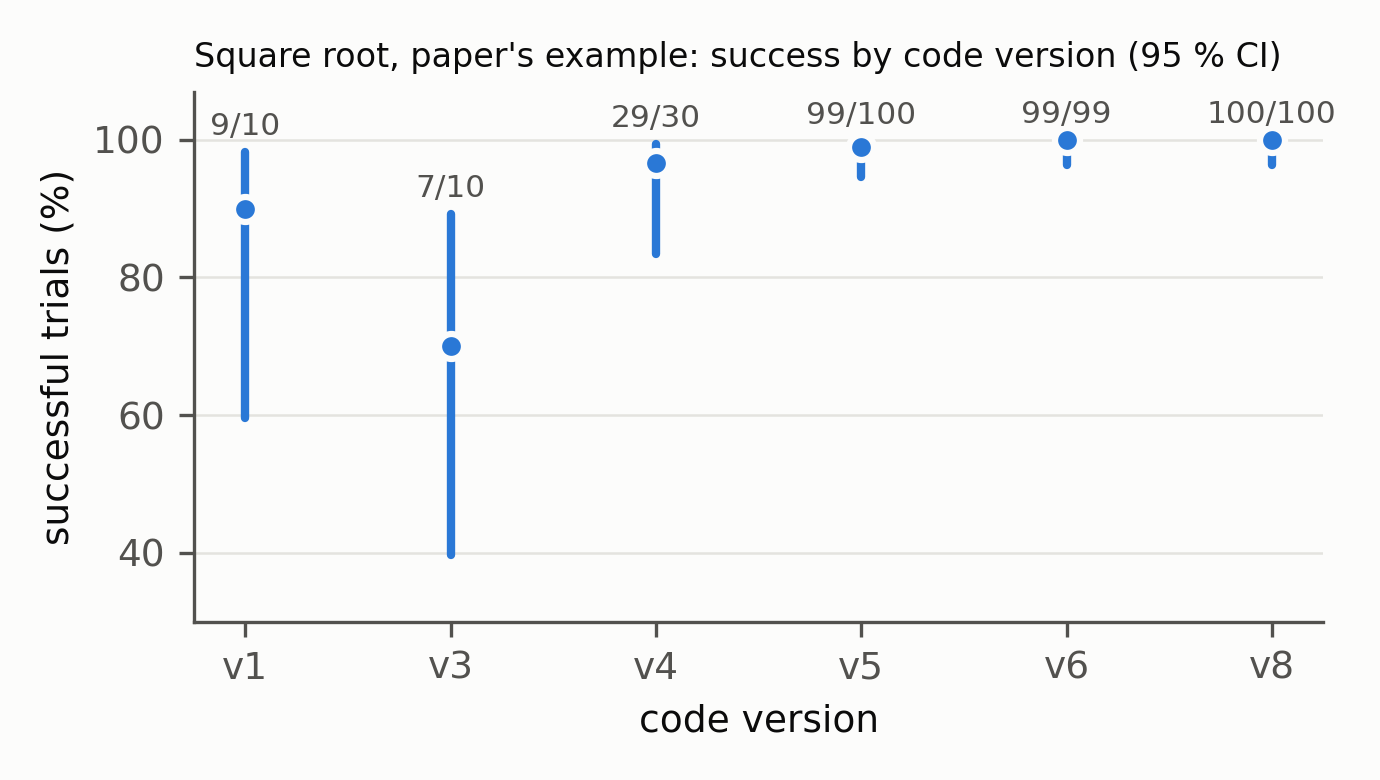
\includegraphics[width=0.48\linewidth]{fig_reliability.png}\hfill
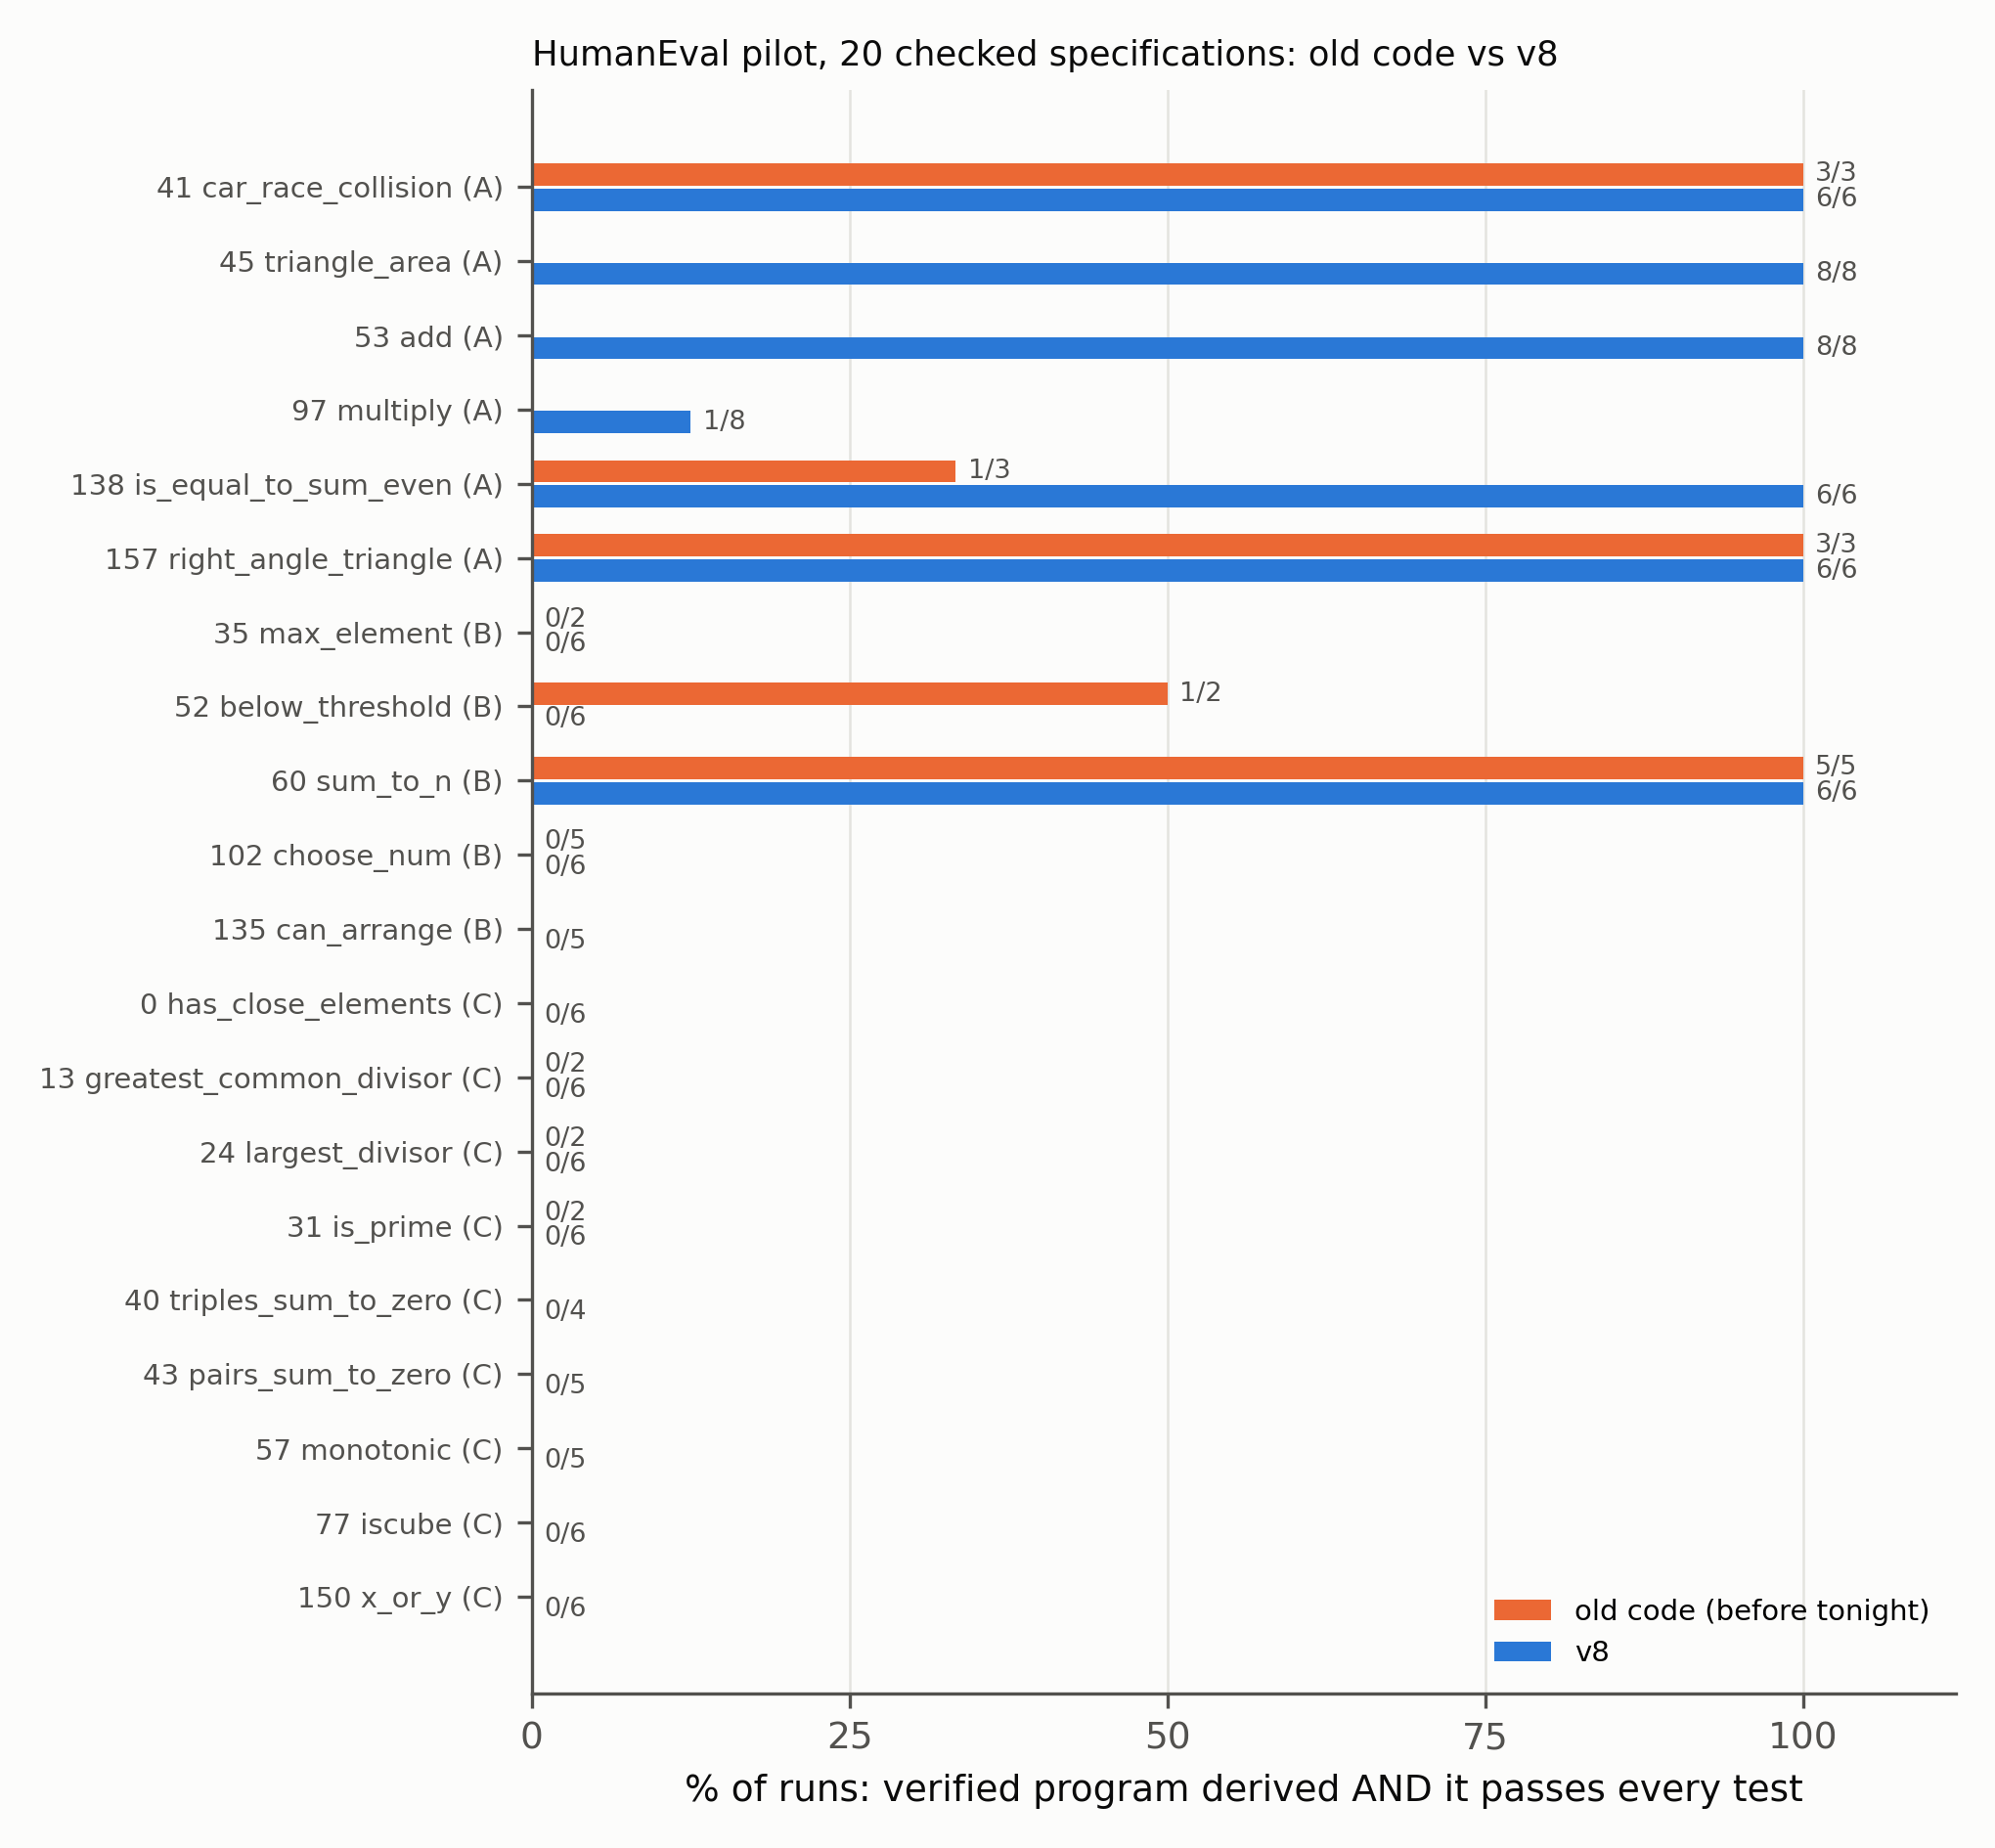
\includegraphics[width=0.5\linewidth]{fig_pilot.png}
\caption{Left: square-root success by code version with Wilson 95\% intervals. Right: HumanEval pilot, runs that derived a verified program that also passes every test, old code vs v8.}
\label{fig:pilot}
\end{figure}

\section{Discussion and limitations}
The paper's improvement over GPT-4 on tests is absorbed by today's model; refinement's value is a guarantee for all inputs and a program that does not degrade from HumanEval to EvalPlus. Coverage (20/164) is limited by the specification language, not by the search. Specifications are ours (checked, but not the paper's); one model family at low effort; proofs say nothing about running time; the leaf assist is not in the paper and is reported on and off.

\section{Related work}
Refinement calculus and correctness-by-construction~\cite{morgan,backwright,corc}; LLMs with verifiers (Refine4LLM~\cite{refine4llm}, Clover~\cite{clover}, Lemur~\cite{lemur}, Baldur~\cite{baldur}); benchmarks~\cite{humaneval,evalplus}; provers~\cite{z3,coqhammer,lean4}.

\begin{thebibliography}{99}
\bibitem{refine4llm} Y.~Cai, Z.~Hóu, D.~Sanán, X.~Luan, Y.~Lin, J.~Sun, J.~S.~Dong. Automated Program Refinement: Guide and Verify Code Large Language Model with Refinement Calculus. Preprint, 2024.
\bibitem{morgan} C.~Morgan. \emph{Programming from Specifications}. Prentice Hall, 2nd ed., 1994.
\bibitem{backwright} R.-J.~Back, J.~von Wright. \emph{Refinement Calculus: A Systematic Introduction}. Springer, 1998.
\bibitem{corc} T.~Runge, I.~Schaefer, L.~Cleophas, T.~Thüm, D.~Kourie, B.~W.~Watson. Tool Support for Correctness-by-Construction. FASE 2019.
\bibitem{clover} C.~Sun, Y.~Sheng, O.~Padon, C.~Barrett. Clover: Closed-Loop Verifiable Code Generation. 2023.
\bibitem{lemur} H.~Wu, C.~Barrett, N.~Narodytska. Lemur: Integrating Large Language Models in Automated Program Verification. ICLR 2024.
\bibitem{baldur} E.~First, M.~Rabe, T.~Ringer, Y.~Brun. Baldur: Whole-Proof Generation and Repair with Large Language Models. ESEC/FSE 2023.
\bibitem{humaneval} M.~Chen et al. Evaluating Large Language Models Trained on Code. 2021.
\bibitem{evalplus} J.~Liu, C.~S.~Xia, Y.~Wang, L.~Zhang. Is Your Code Generated by ChatGPT Really Correct? NeurIPS 2023.
\bibitem{z3} L.~de~Moura, N.~Bjørner. Z3: An Efficient SMT Solver. TACAS 2008.
\bibitem{coqhammer} Ł.~Czajka, C.~Kaliszyk. Hammer for Coq: Automation for Dependent Type Theory. JAR 2018.
\bibitem{lean4} L.~de~Moura, S.~Ullrich. The Lean 4 Theorem Prover and Programming Language. CADE 2021.
\end{thebibliography}
\end{document}
